\documentclass[newPxFont]{beamer}
%\documentclass[handout]{beamer} % Раздаточный материал (на слайдах всё сразу)
%\documentclass[aspectratio=169]{beamer} % Соотношение сторон


\usetheme{LTX}

%-=-=-=-=-=-=-=-=-=-=-=-=-=-=-=-=-=-=-=-=-=-=-=-=
%        LOADING PACKAGES
%-=-=-=-=-=-=-=-=-=-=-=-=-=-=-=-=-=-=-=-=-=-=-=-=
\usepackage[T2A]{fontenc}			% кодировка
\usepackage[utf8]{inputenc}			% кодировка исходного текста
\usepackage[english,russian]{babel}	% локализация и переносы


%%% Дополнительная работа с математикой
\usepackage{amsmath,amsfonts,amssymb,amsthm,mathtools} % AMS

%%% Работа с картинками
\usepackage{graphicx}  % Для вставки рисунков
\graphicspath{{images/}{images2/}}  % папки с картинками
\setlength\fboxsep{3pt} % Отступ рамки \fbox{} от рисунка
\setlength\fboxrule{1pt} % Толщина линий рамки \fbox{}
\usepackage{wrapfig} % Обтекание рисунков текстом

%%% Работа с таблицами
\usepackage{array,tabularx,tabulary,booktabs} % Дополнительная работа с таблицами
\usepackage{longtable}  % Длинные таблицы
\usepackage{multirow} % Слияние строк в таблице

%%% Программирование
\usepackage{etoolbox} % логические операторы

%%% Другие пакеты
\usepackage{multicol} % Несколько колонок

%%% Картинки
\usepackage{tikz} % Работа с графикой
\usepackage{pgfplots}
\usepackage{pgfplotstable}


\usepackage{xcolor}
\usepackage{hyperref}
\usepackage{verbatim}
\usepackage{fancyvrb}
\usepackage{mdframed}

\usepackage{chronology}

\renewcommand{\event}[3][e]{%
  \pgfmathsetlength\xstop{(#2-\theyearstart)*\unit}%
  \ifx #1e%
    \draw[fill=black,draw=none,opacity=0.5]%
      (\xstop, 0) circle (.2\unit)%
      node[opacity=1,rotate=45,right=.2\unit] {#3};%
  \else%
    \pgfmathsetlength\xstart{(#1-\theyearstart)*\unit}%
    \draw[fill=black,draw=none,opacity=0.5,rounded corners=.1\unit]%
      (\xstart,-.1\unit) rectangle%
      node[opacity=1,rotate=45,right=.2\unit] {#3} (\xstop,.1\unit);%
  \fi}%

\title{Уютный факультатив по \LaTeX}
\subtitle{Введение в \LaTeX}
\date{\today}

\begin{document}

 \maketitle
 
 
\begin{frame}
\frametitle{Что это вообще такое ?} 

\alert{TeX} --- это созданная американским математиком и программистом Дональдом Кнутом система для верстки текстов с формулами. 


\end{frame} 

\begin{frame}
\frametitle{Почему \LaTeX{}?} 
\begin{itemize}
\item Он позволяет делать красивые документы
\item Особенно документы с формулами
\item Он был создан учёными для учёных
\item Большое и активное комьюнити, у которого всегда можно попросить о помощи
\item Он уютный!
\item Многие вещи, связанные с оформлением автоматизированы, что позволяет думать о содержании
\item Огромное количество различных пакетов и расширений в свободном доступе
\end{itemize}
\end{frame}




\begin{frame}
\frametitle{Откуда появился \LaTeX{}?} 
\begin{columns}
\begin{column}{.48\linewidth}
\centering 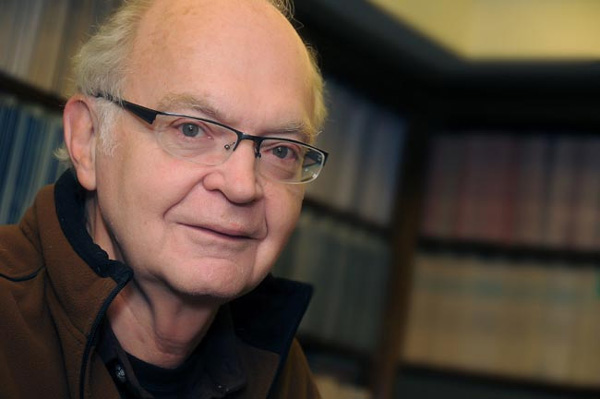
\includegraphics[scale=0.2]{DK.jpg}\\
\mbox{ } \\
Дональд Кнут создал в 1978 году программу \TeX.		
\end{column}

\begin{column}{.48\linewidth}
\centering Лесли Лэмпорт создал в 1984 году макропакет \LaTeX. \\
\mbox{ } \\
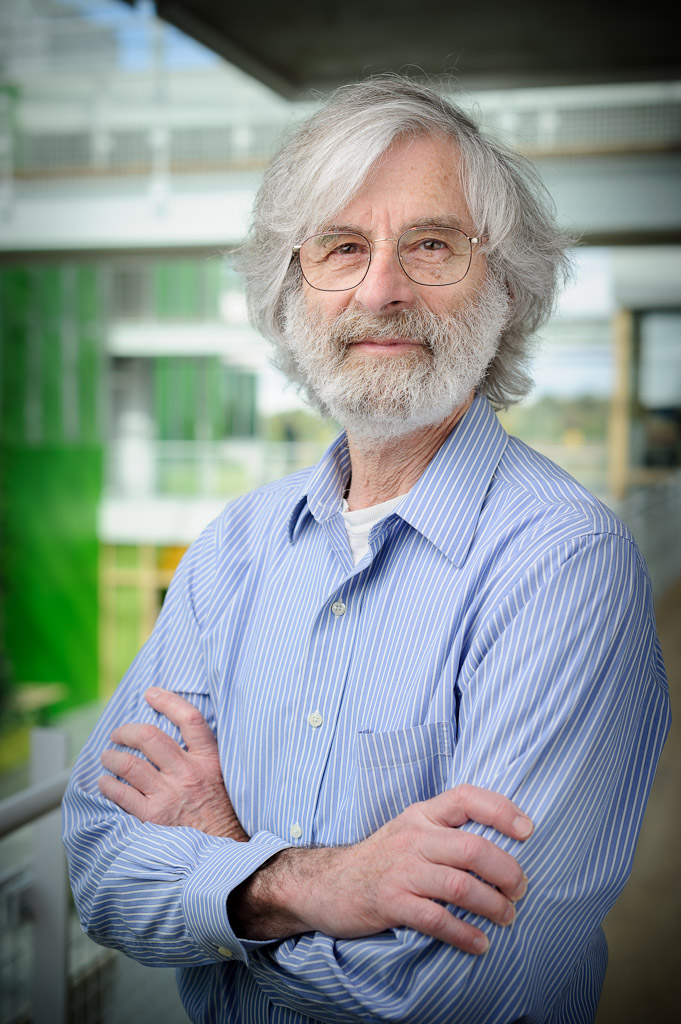
\includegraphics[scale=0.4]{LL.jpg}		
\end{column}
\end{columns}
\end{frame}



\begin{frame}
\frametitle{Особенности \LaTeX}
\LaTeX{} не WYSIWYG (What You See Is What You GET)
В WYSIWYG системах что автор видит на экране, то и получается на печати.

\mbox{ } 

\LaTeX{} WYSIWYM (What You See Is What You {\color{green} MEAN})
\LaTeX{} сам позаботится об оформлении, вам остаётся только думать о содержании!
\end{frame}



\begin{frame}[fragile]
\frametitle{Как это работает?}
Вы пишите свой текст с различными {\color{green} командами}, описывающими структуру текста, а \LaTeX{} преобразует их в красиво отформатированный pdf-документ!

\begin{mdframed}[backgroundcolor=LTXLightGreen]
В Португалии \verb|\textbf|\{дождь\} является \verb|\textit|\{причиной\}  не выходить на работу.
\end{mdframed}

\centering
   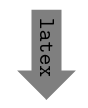
\includegraphics[scale=0.3]{fuc.png}%}

\begin{mdframed}[backgroundcolor=LTXLightGreen] 
В Португалии \textbf{дождь} является \textit{причиной} не выходить на работу.
\end{mdframed}   
\end{frame}

\begin{frame}[fragile]
\frametitle{Ещё примеры работы \LaTeX{}!} 

\begin{tabular}{p{5.5cm}p{4cm}}
\vspace{10mm} \verb|includegraphics[scale=0.15]{doge.png}| &  \begin{center} 
\includegraphics[scale=0.15]{doge.png} \end{center}
\end{tabular}
\begin{tabular}{p{5.5cm}p{4cm}}
\centering \verb|$\alpha^{x}+\sigma_{t}$| & \centering  $\alpha^{x}+\sigma_{t}$
\end{tabular}
\begin{tabular}{p{6.5cm}p{4cm}}
\begin{verbatim}
\begin{enumerate}
	\item Чай
	\item Молоко
\end{enumerate}
\end{verbatim} 
& \vspace{6mm} \begin{center}
\begin{enumerate}
	\item Чай
	\item Молоко
\end{enumerate}	 
\end{center} 
\end{tabular}
\end{frame}


\begin{frame}[fragile]
\frametitle{Любой документ состоит из двух частей!} 
\begin{mdframed}[backgroundcolor=LTXLightGreen] 
\verb|\documentclass[pdftex, 12pt, a4paper]{article}|\\
\\
\% Тут располагается преамбула документа!\\
\\
\verb|\begin{document}|\\
\\
\% Тут располагается сам документ!\\
\\
\verb|\{document}|\\
\end{mdframed}    
\end{frame}


\begin{frame}[fragile]
\frametitle{Хорошие мысли о \LaTeX!} 
\begin{itemize}
\item Каждый документ состоит из преамбулы и основной части;
\item Все {\color{green} комнады} начинаются с знака \verb|\|;
\item Каждый аргумент команды стоит в фигурных скобках \{ \};
\item С помощью знака \% можно закомментировать какую-то часть документа, \LaTeX{} проигнорирует закомментированную часть;
\item Неважно сколько строк я оставил между абзацами и сколько пробелов я оставил между словами; 
\end{itemize}
\end{frame}

\begin{frame}[fragile]
\frametitle{Формулы в \LaTeX!} 
\begin{itemize}
\item С помощью символа \$ мы можем перейти внутри текста в математический режим! Один \$ открывает математический режим, второй закрывает его! 
\item С помощью символов \$\$ или \verb|\[| и \verb|\]| можно написать выключную формулу. Выключной объект --- такой объект, для которого необходима отдельная строка!
\item Внутри математического режима \LaTeX{} сам расставляет пробелы. Все ваши пробелы игнорируются.
\end{itemize}
\end{frame}

\begin{frame}
\frametitle{Формулы в \LaTeX!} 
\begin{itemize}
\item В \LaTeX{} можно найти символы на все случаи жизни $\Im$
\item По {\color{blue} \href{http://detexify.kirelabs.org/classify.html}{этой ссылке}} расположен распознаватель символов!
\item В книге Львовского есть огровное количество символов с подробными комментариями! Например: 
\centering  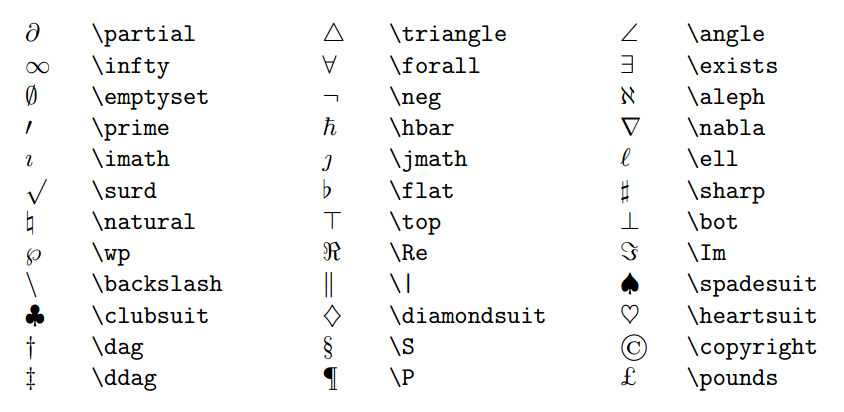
\includegraphics[scale=0.2]{table.png}
\end{itemize}
\end{frame}


\begin{frame}
\frametitle{Служебные символы} 

\mbox{ } 

\centering
\Large{ \$ \% \{ \} \# \& --- служебные символы}

\mbox{ }

\begin{itemize}
\item \normalsize{Чтобы использовать \$ или другой символ в тексте, надо написать $\setminus$\$.}
\end{itemize}
\end{frame}


\section{Мотивация}

\begin{frame}
\centering
\frametitle{Мотивация изучать \LaTeX{}} 
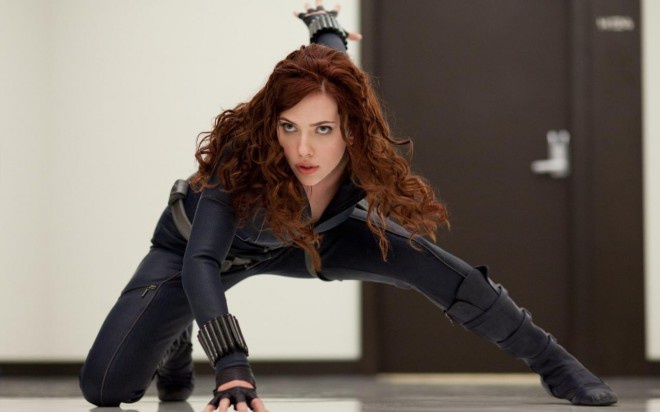
\includegraphics[scale=0.48]{scarlet.jpg}

\end{frame}


\begin{frame}
\frametitle{\insertsection} 

	\centering
    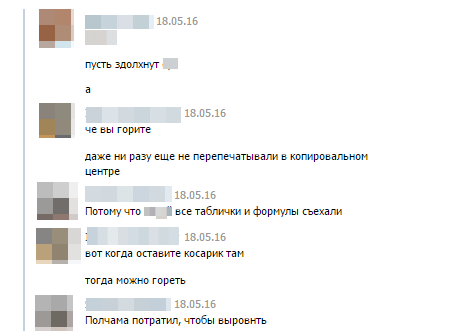
\includegraphics[height=0.7\textheight]{m1.png}
    
    
    \alert{\textbf{В \LaTeX{} никогда ничего никуда не съедет!}}
    
    
\end{frame}

\begin{frame}
\frametitle{\insertsection} 
    \centering
    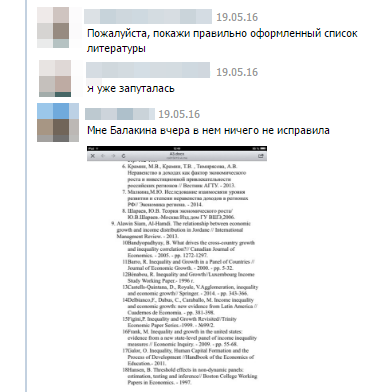
\includegraphics[height=0.7\textheight]{m2.png}
    
    \vfill
    \alert{\textbf{В \LaTeX{} список литературы сгенерируется автоматически!}}
\end{frame}

\begin{frame}
\frametitle{\insertsection} 
    \centering
    
\includegraphics[height=0.7\textheight]{m4.png}
    
    \vfill
    \alert{\textbf{Зачем первак, когда есть \LaTeX{}!}}
\end{frame}


\begin{frame}
\frametitle{\insertsection} 
    \centering
    
\includegraphics[scale=0.5]{m5.png}
    
    \vfill
    \alert{\textbf{В \LaTeX{} можно написать абсолютно любой шаблон!}}
\end{frame}


\begin{frame}
\frametitle{\insertsection} 
    \centering
    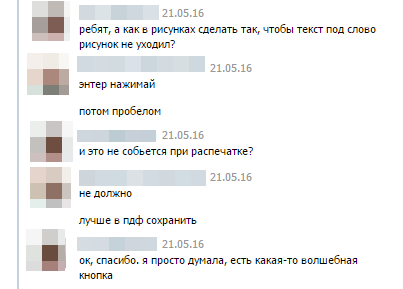
\includegraphics[height=0.6\textheight]{m6.png}
    
    \vfill
    \alert{\textbf{В \LaTeX{} вы навсегда забудете о <<сначала энтер, потом 4 раза пробел>>!}}
\end{frame}


\begin{frame}
\frametitle{\insertsection} 
    \centering
    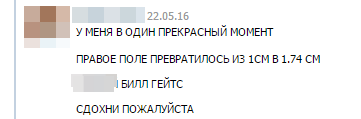
\includegraphics[scale=0.5]{m7.png}

	\mbox{ }     
     
    
\includegraphics[scale=0.6]{m9.png}
    
    \vfill
    \alert{\textbf{Проблемы при распечатке? Никогда не слышал!}}
\end{frame}


\begin{frame}
\frametitle{\insertsection} 
    \centering
    
\includegraphics[scale=0.5]{m8.png}
    
    \vfill
    \alert{\textbf{В \LaTeX{} ничего не изменится и не исчезнет без вашего ведома!}}
\end{frame}


\begin{frame}
\frametitle{\insertsection} 
    \centering
    
\includegraphics[scale=0.5]{m10.png}
    
    \vfill
    \alert{\textbf{А ещё то ли \LaTeX{} то ли ГОСТ придумали рептилоиды!}}
\end{frame}


\begin{frame}
\frametitle{А если говорить серьёзно, то \ldots} 
    \centering
    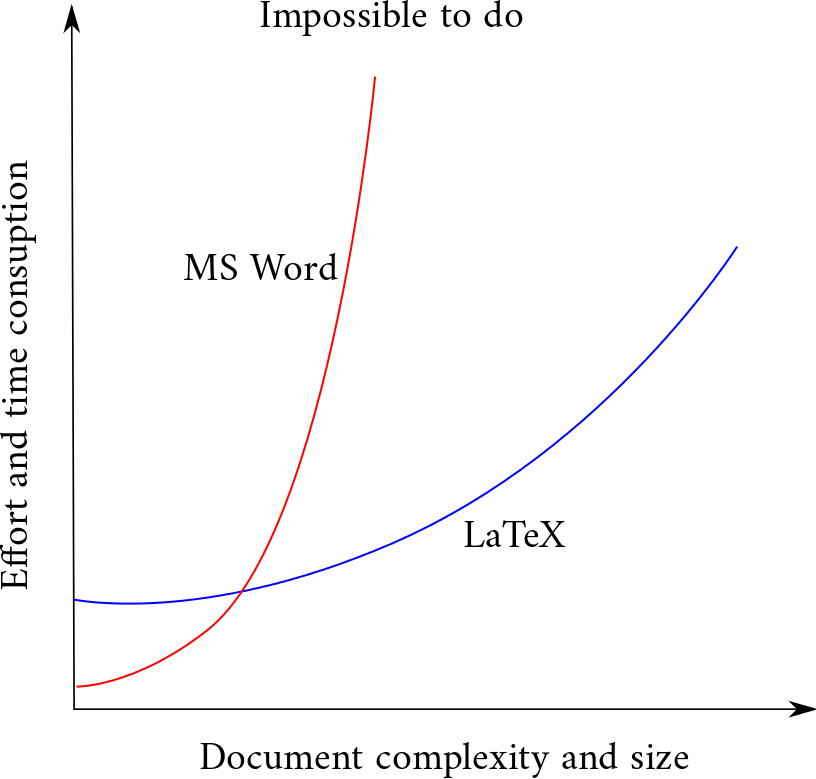
\includegraphics[scale=0.2]{latexvsword.png}
\end{frame}


\section{Домашка}

\begin{frame}[fragile]
\frametitle{\insertsection} 
\begin{enumerate}
\item Зайти на страничку курса в Github по вот {\color{blue} \href{https://github.com/FUlyankin/LaTeX/wiki}{этой ссылке}} и внимательно изучить её! 
\item Установить \LaTeX{}! Как? Смотри в репозитории! 
\item Создать свой первый документ в \LaTeX! Создать в нём перечень с       десятью фактами о себе. Написать три своих любимых формулы и одну ненавистную.      Рассказать почему эти формулы любимые, а та ненавистная. Вставить своё фото!  Не забыть подключить в преамбуле пакет для вставки картинок с помощью команды \verb|\usepackage|\{graphicx\}!
\end{enumerate}
\end{frame}


\end{document}

%\only<2->{Эта строчка появляется не сразу и не занимает места.
    %\centering
    %
\includegraphics[height=0.7\textheight]{rep.jpg}


\begin{frame}[fragile]

\end{frame}